\chapter{Исследовательский раздел}
Для проверки работоспособности методов распределения памяти был использован тест производительности для аллокаторов от разработчика библиотеки rpmalloc\cite{rpmalloc-bench}. В качестве параметров задаются: количество потоков, распределение размеров объектов, количество освобождений памяти из разных потоков, количество циклов в каждом потоке, количество аллокаций в каждом потоке, количество итераций на одну операцию, начальный и конечный размеры блоков. Все методы сравниваются по двум параметрам, количество операций в секунду и процент накладных расходов относительно запрошенной памяти к выделенной.

\section{Используемое аппаратное обеспечение}
Тесты производительности запускались на процессоре AMD Ryzen 1400  с частотой 3.2 МГц. Данный процессор имеет 4 физических ядра и 8 логических ядер. Для процессоров AMD серии Ryztn важна скорость оперативной памяти, потому что от нее напрямую зависит частота шины infinity fabric\cite{infinity-fabric}, которая отвечает за транспорт данных между компонентами. В данной работе использовалась память стандарта DDR4 разогнанная до частоты 3466 МГц.

\section{Используемое программное обеспечение}
В качестве целевого ПО для сравнения библиотек была использована ОС Linux с ядром версии 5.11.6, которое является последним на момент проведения тестирования.

\section{Сравнение методов распределения памяти}
Все методы проверялись на разных размерах, чтобы протестировать распределение памяти для разных типов объектов.  Всего было проведено 5 серий тестов с количеством потоков от 1 до 16. Каждый тест имеет свои параметры, чтобы полностью охватить все возможные случаи использования методов.

\begin{figure}[!h]
	\begin{center}
		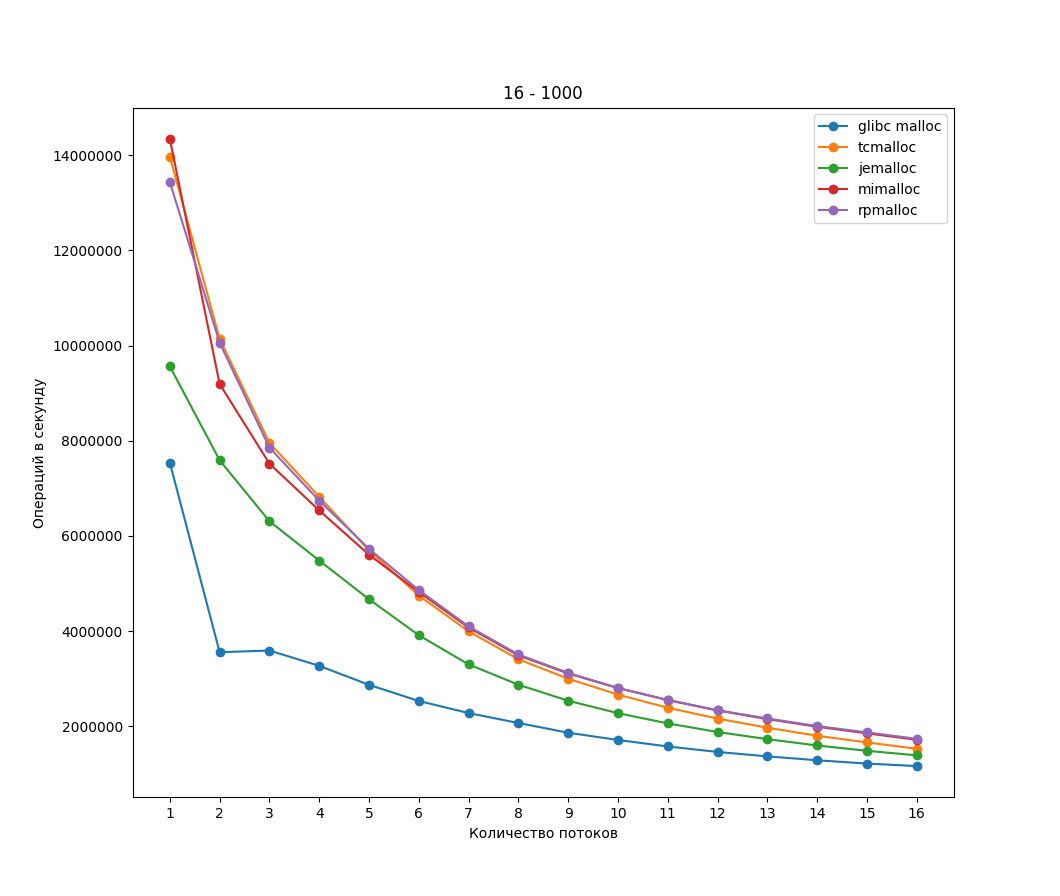
\includegraphics[width=1.0\linewidth, height=0.37\textheight]{images/16_1000_ops.png}
		\caption{Количество операций в секунду для размеров от 16 до 1000 байт.}
		\label{16_1000_ops}
	\end{center}
\end{figure}

\begin{figure}[!h]
	\begin{center}
		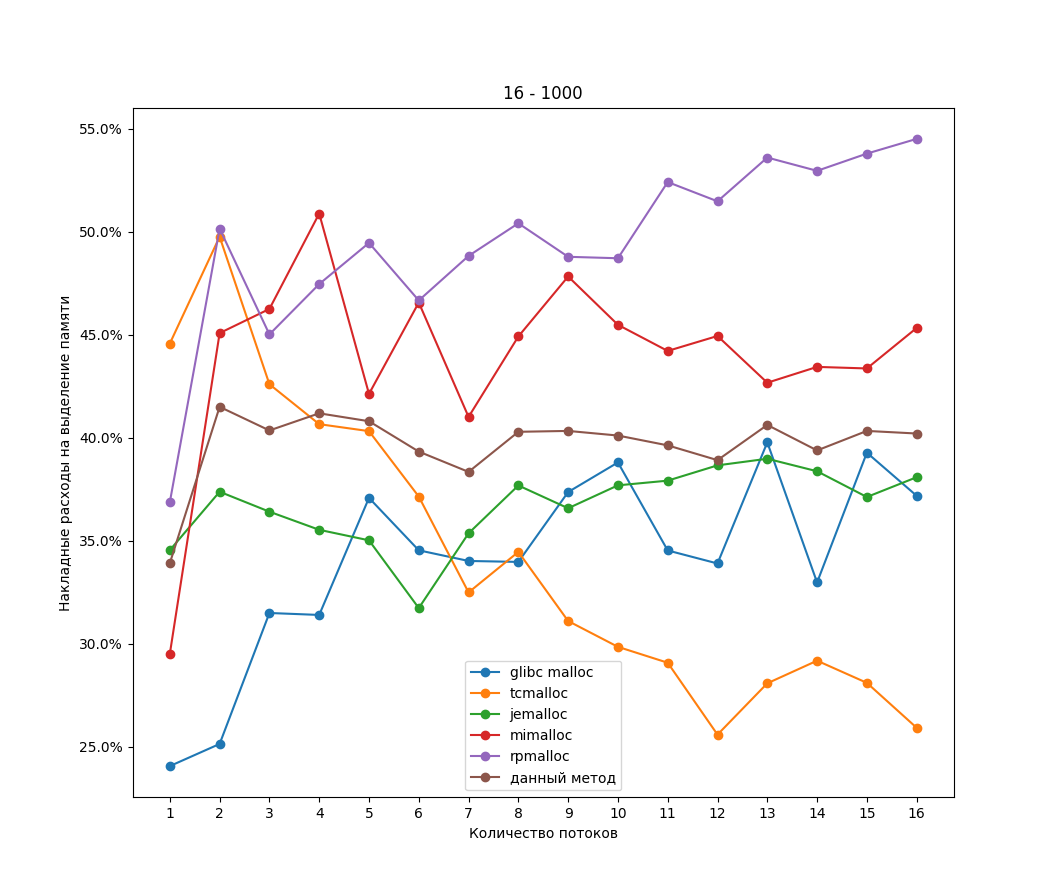
\includegraphics[width=1.0\linewidth, height=0.37\textheight]{images/16_1000_overhead.png}
		\caption{Процент накладных расходов для размеров от 16 до 1000 байт.}
		\label{16_1000_overhead}
	\end{center}
\end{figure}

\begin{figure}[!h]
	\begin{center}
		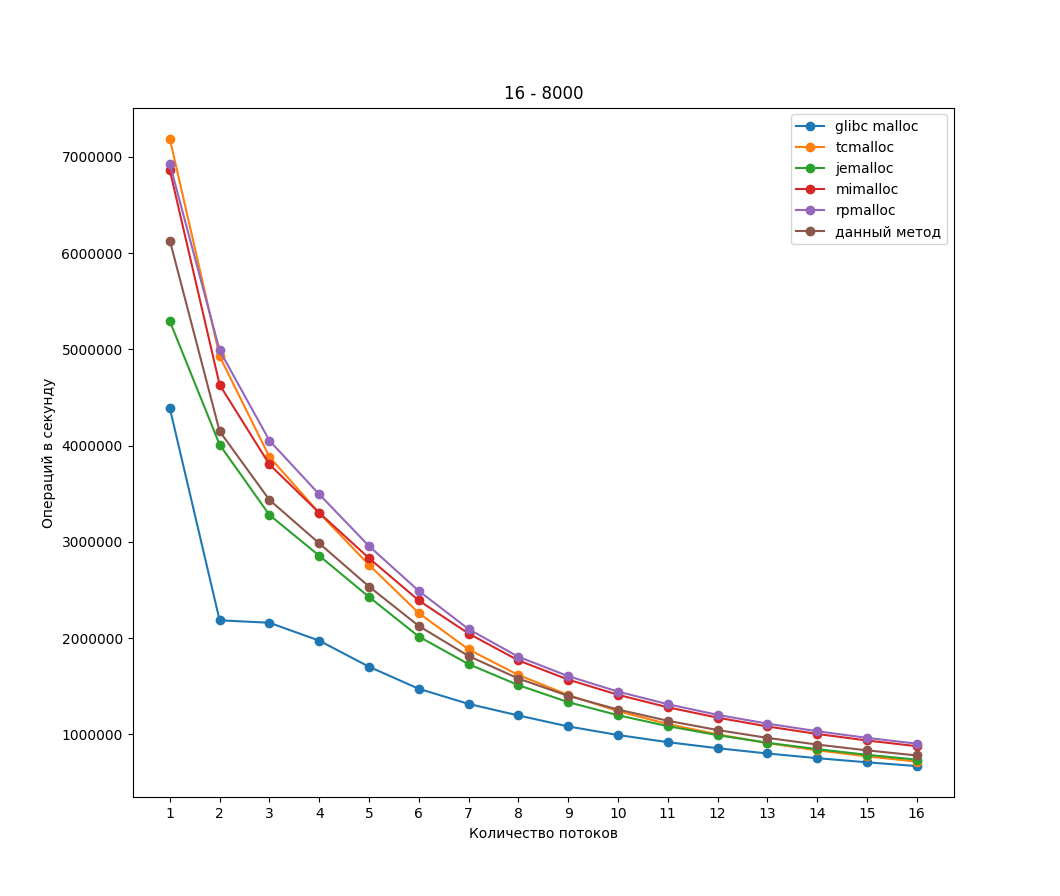
\includegraphics[width=1.0\linewidth, height=0.37\textheight]{images/16_8000_ops.png}
		\caption{Количество операций в секунду для размеров от 16 до 8000 байт.}
		\label{16_8000_ops}
	\end{center}
\end{figure}

\begin{figure}[!h]
	\begin{center}
		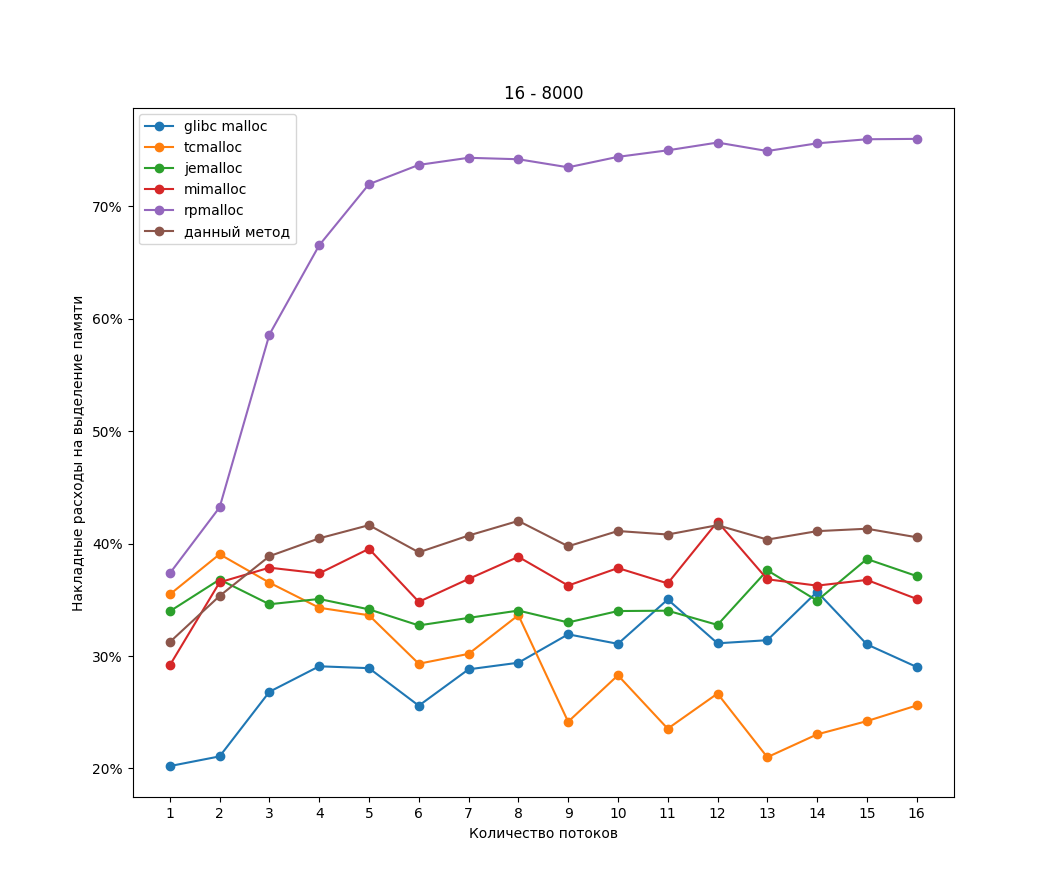
\includegraphics[width=1.0\linewidth, height=0.37\textheight]{images/16_8000_overhead.png}
		\caption{Процент накладных расходов для размеров от 16 до 8000 байт.}
		\label{16_8000_overhead}
	\end{center}
\end{figure}

\begin{figure}[!h]
	\begin{center}
		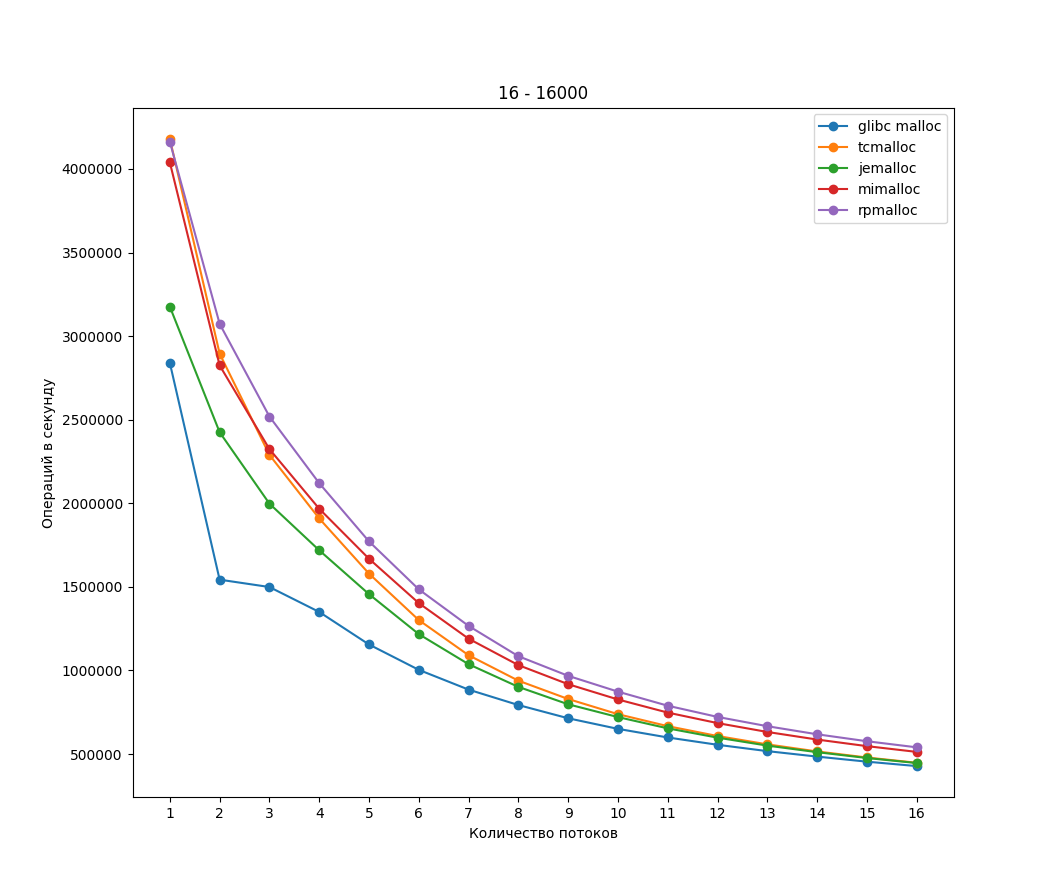
\includegraphics[width=1.0\linewidth, height=0.37\textheight]{images/16_16000_ops.png}
		\caption{Количество операций в секунду для размеров от 16 до 16000 байт.}
		\label{16_16000_ops}
	\end{center}
\end{figure}

\begin{figure}[!h]
	\begin{center}
		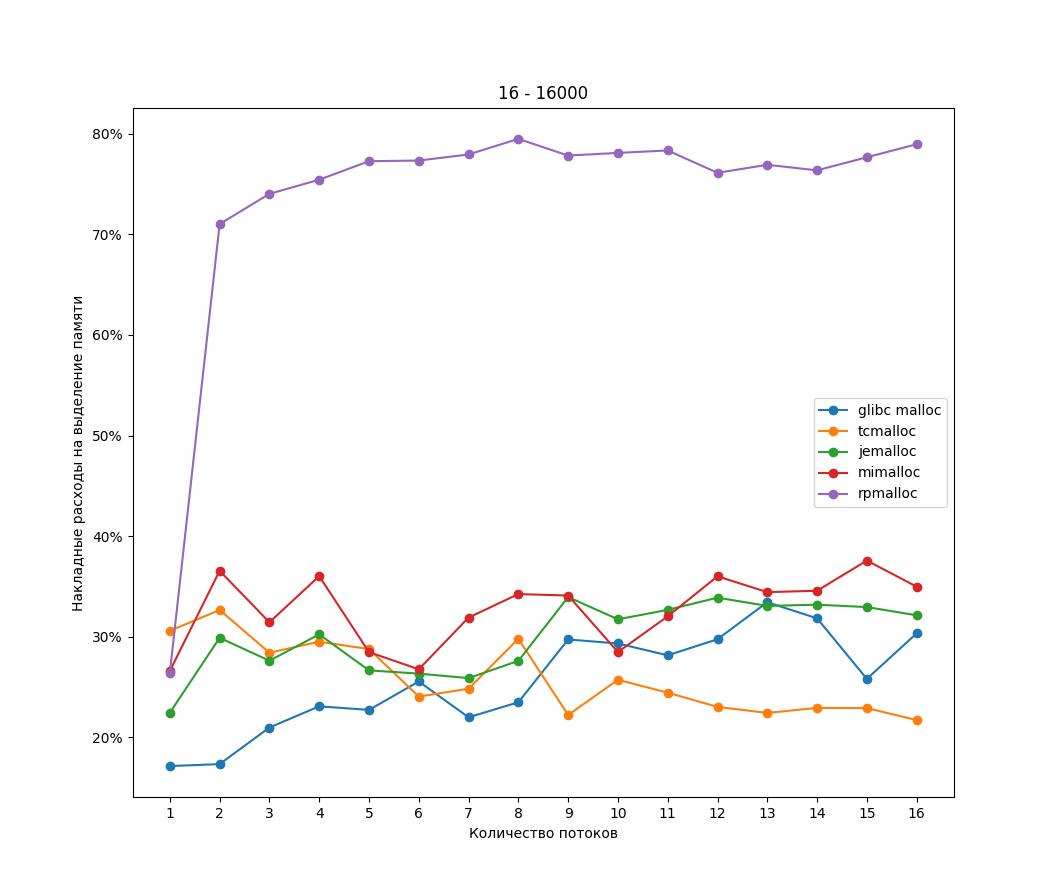
\includegraphics[width=1.0\linewidth, height=0.37\textheight]{images/16_16000_overhead.png}
		\caption{Процент накладных расходов для размеров от 16 до 16000 байт.}
		\label{16_16000_overhead}
	\end{center}
\end{figure}

\begin{figure}[!h]
	\begin{center}
		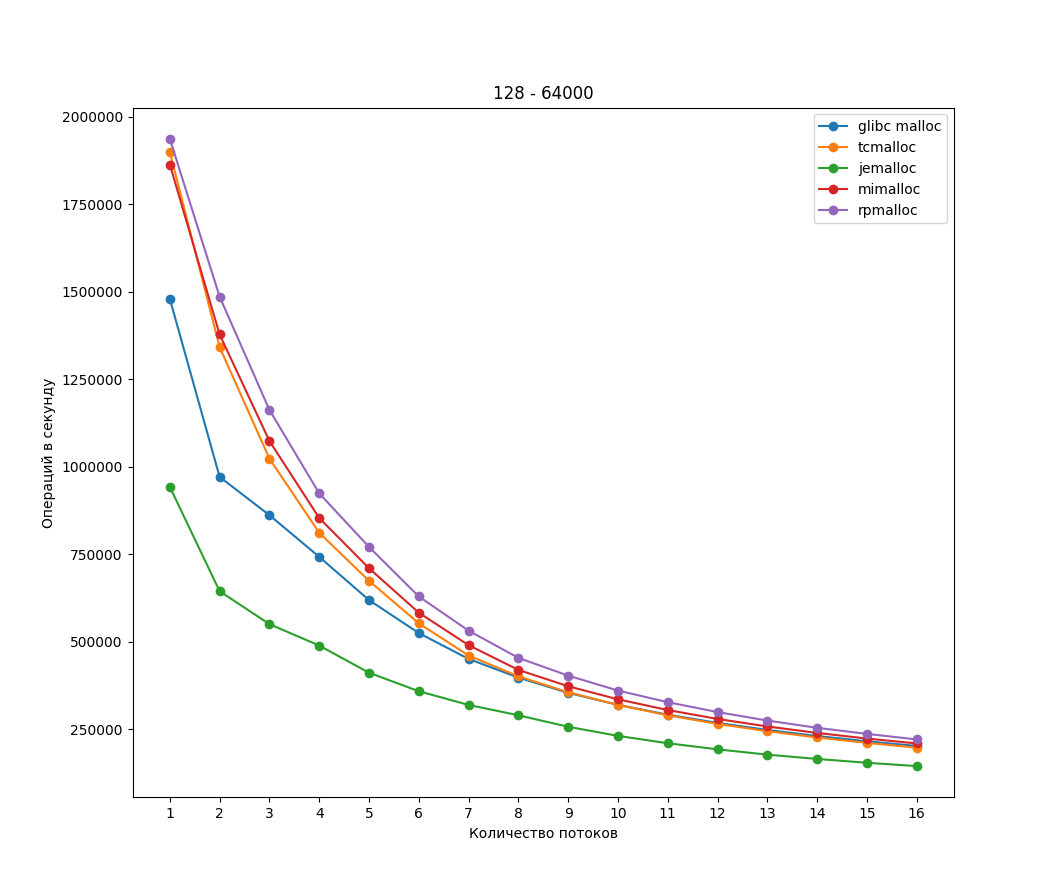
\includegraphics[width=1.0\linewidth, height=0.37\textheight]{images/128_64000_ops.png}
		\caption{Количество операций в секунду для размеров от 128 до 64000 байт.}
		\label{128_64000_ops}
	\end{center}
\end{figure}

\begin{figure}[!h]
	\begin{center}
		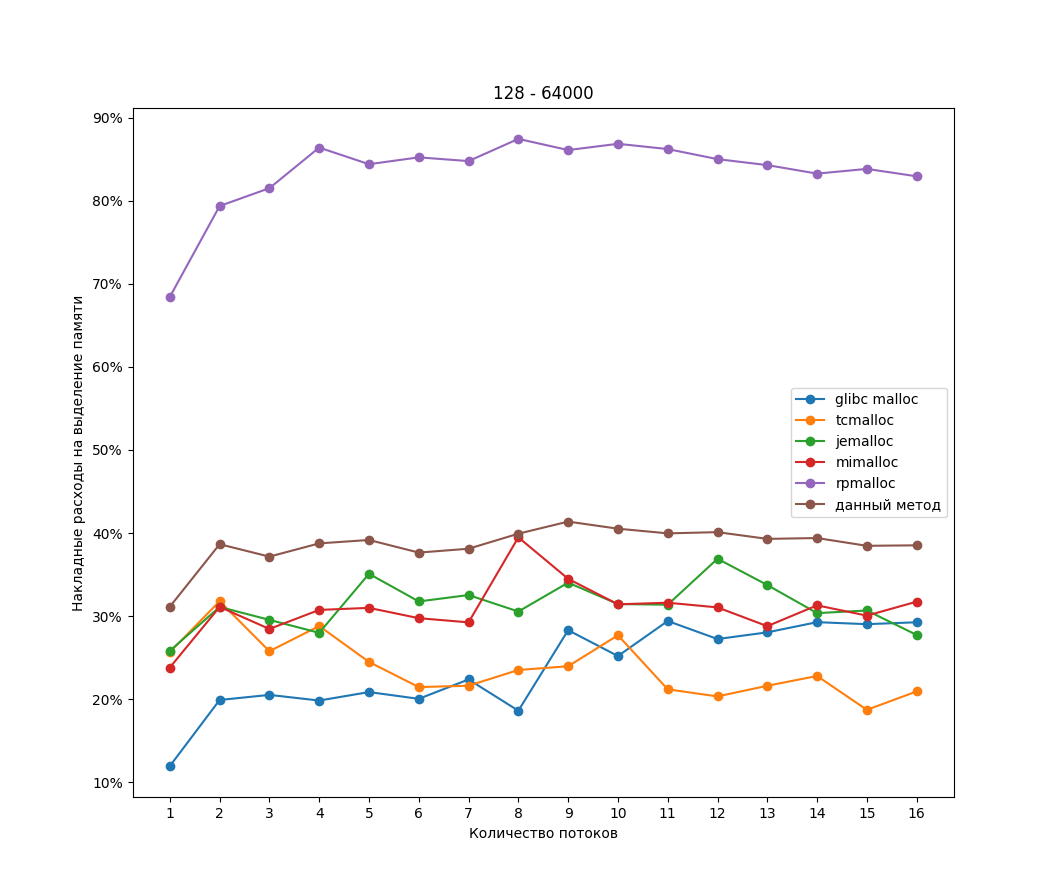
\includegraphics[width=1.0\linewidth, height=0.37\textheight]{images/128_64000_overhead.png}
		\caption{Процент накладных расходов для размеров от 128 до 64000 байт.}
		\label{128_64000_overhead}
	\end{center}
\end{figure}

\begin{figure}[!h]
	\begin{center}
		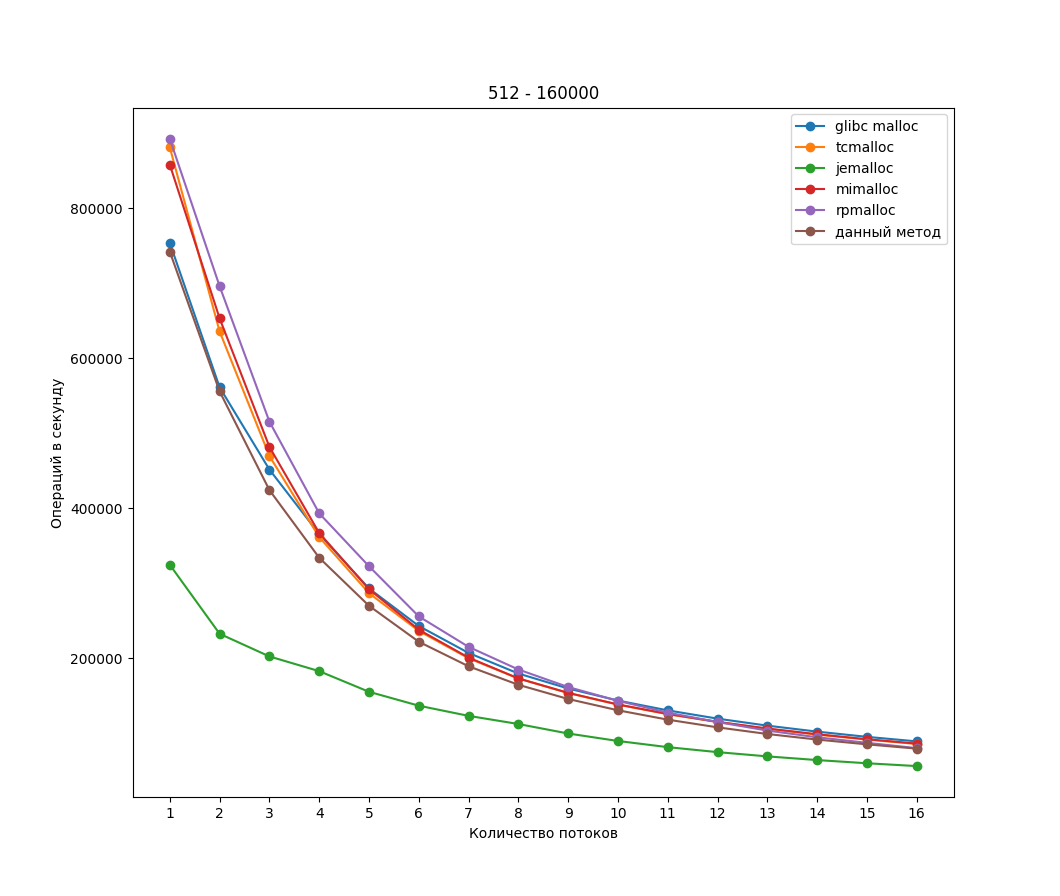
\includegraphics[width=1.0\linewidth, height=0.37\textheight]{images/512_160000_ops.png}
		\caption{Количество операций в секунду для размеров от 512 до 160000 байт.}
		\label{512_160000_ops}
	\end{center}
\end{figure}

\begin{figure}[!h]
	\begin{center}
		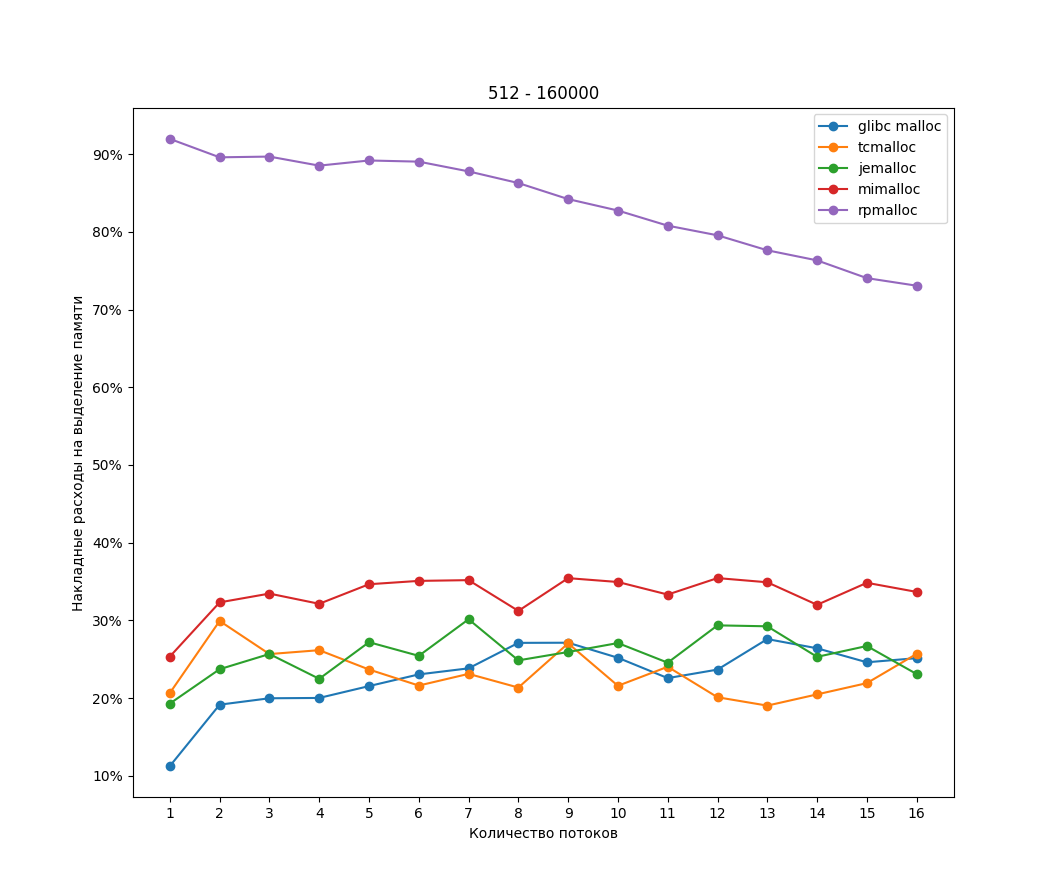
\includegraphics[width=1.0\linewidth, height=0.37\textheight]{images/512_160000_overhead.png}
		\caption{Процент накладных расходов для размеров от 512 до 160000 байт.}
		\label{512_160000_overhead}
	\end{center}
\end{figure}

Исходя из полученных результатов метрик количества запросов в секунду (рисунки \ref{16_1000_ops}, \ref{16_8000_ops}, \ref{16_16000_ops}, \ref{128_64000_ops}, \ref{512_160000_ops}) и процента накладных расходов (рисунки \ref{16_1000_overhead}, \ref{16_8000_overhead}, \ref{16_16000_overhead}, \ref{128_64000_overhead}, \ref{512_160000_overhead}), можно рекомендовать данный метод для использования в качестве распределителя памяти для приложений.

%%% Local Variables:
%%% mode: latex
%%% TeX-master: "rpz"
%%% End: